%%%%%%%%%%%%%%%%%%%%%%%%%%%%%%%%%%%%%%%%%
% NIWeek 2014 Poster by T. Reveyrand
% www.microwave.fr
% http://www.microwave.fr/LaTeX.html
% ---------------------------------------
%
% Original template created by:
% Brian Amberg (baposter@brian-amberg.de)
%
% This template has been downloaded from:
% http://www.LaTeXTemplates.com
%
% License:
% CC BY-NC-SA 3.0 (http://creativecommons.org/licenses/by-nc-sa/3.0/)
%
%%%%%%%%%%%%%%%%%%%%%%%%%%%%%%%%%%%%%%%%%

%----------------------------------------------------------------------------------------
%   PACKAGES AND OTHER DOCUMENT CONFIGURATIONS
%----------------------------------------------------------------------------------------

\documentclass[a0paper,portrait]{baposter}

\usepackage[font=small,labelfont=bf]{caption} % Required for specifying captions to tables and figures
\usepackage{booktabs} % Horizontal rules in tables
\usepackage{relsize} % Used for making text smaller in some places

\usepackage{amsmath,amsfonts,amssymb,amsthm} % Math packages
\usepackage{eqparbox}
\usepackage{textcomp}
\usepackage{caption}
\usepackage{subcaption}
\usepackage{graphicx}
\usepackage{listings}
\usepackage{mathtools}
\usepackage{multirow}
\usepackage[percent]{overpic}
%\usepackage{hyperref}

%\usepackage{pgf}

\usepackage[utf8]{inputenc}
\usepackage{tikz}
\usetikzlibrary{calc}
\usetikzlibrary{shapes,arrows}
\usetikzlibrary{arrows,automata}
\usetikzlibrary{positioning}
\usetikzlibrary{shapes.callouts}


\usepackage{multicol}
\usepackage{hyperref}
\usepackage[font=small,labelfont=bf]{caption}
\usepackage{makecell}
\usepackage{enumitem}
\usepackage{fontawesome}
\usepackage{xparse}


\newcommand{\tikzmark}[1]{\tikz[overlay,remember picture] \node (#1) {};}
\def\Put(#1,#2)#3{\leavevmode\makebox(0,0){\put(#1,#2){#3}}}

%\tikzset{
%    invisible/.style={opacity=0,text opacity=0},
%    visible on/.style={alt=#1{}{invisible}},
%    alt/.code args={<#1>#2#3}{%
%      \alt<#1>{\pgfkeysalso{#2}}{\pgfkeysalso{#3}} % \pgfkeysalso doesn't change the path
%    },
%}

\NewDocumentCommand{\mycallout}{r<> O{opacity=0.8,text opacity=1} m m}{%
\tikz[remember picture, overlay]\node[align=center, fill=cyan!20, text width=3.5cm,
#2, rounded corners,
draw,rectangle callout,anchor=pointer,callout relative pointer={(230:1cm)}]
at (#3) {#4};
}

\renewcommand\theadalign{bc}
\renewcommand\theadfont{\bfseries}
\renewcommand\theadgape{\Gape[4pt]}
\renewcommand\cellgape{\Gape[4pt]}

%for [[ ]]
\usepackage{stmaryrd}

\setlist[itemize]{leftmargin=*}

\graphicspath{{figures/}} % Directory in which figures are stored

 \definecolor{bordercol}{RGB}{40,40,40} % Border color of content boxes
 \definecolor{headercol1}{RGB}{210,235,250} % Background color for the header in the content boxes (left side)
 \definecolor{headercol2}{RGB}{210,235,250} % Background color for the header in the content boxes (right side)
 \definecolor{headerfontcol}{RGB}{0,0,0} % Text color for the header text in the content boxes
 \definecolor{boxcolor}{RGB}{240,255,255} % Background color for the content in the content boxes

\tikzset{
    state/.style={
           ellipse,
           draw=black, thin,
           minimum height=0.5cm,
           minimum width=0.6cm,
           text centered,
           font=\scriptsize
           },
    horiz/.style={
           % font=\tiny,
           inner sep=3pt,
           font=\bf

           } ,
    point/.style={
           circle,
           minimum width = 5pt,
           fill
           }
}

\begin{document}

\setlength{\fboxsep}{0pt}

\background{ % Set the background to an image (background.pdf)
\begin{tikzpicture}[remember picture,overlay]
\draw (current page.north west)+(-2em,2em) node[anchor=north west]
{\includegraphics[height=1.1\textheight]{background}};
\end{tikzpicture}
}

\begin{poster}{
grid=false,
columns=12, % because reasons
borderColor=bordercol, % Border color of content boxes
headerColorOne=headercol1, % Background color for the header in the content boxes (left side)
headerColorTwo=headercol2, % Background color for the header in the content boxes (right side)
headerFontColor=headerfontcol, % Text color for the header text in the content boxes
boxColorOne=boxcolor, % Background color for the content in the content boxes
headershape=rectangle, % Specify the rounded corner in the content box headers
headerfont=\Large\sf\bf, % Font modifiers for the text in the content box headers
textborder=none,
background=none,
headerborder=none, % Change to closed for a line under the content box headers
boxshade=plain
}
{
\includegraphics[width=4cm]{figures/icfp.png}}
%
%----------------------------------------------------------------------------------------
%   TITLE AND AUTHOR NAME
%----------------------------------------------------------------------------------------
%
{\bf \huge{Distilling Sparse Linear Algebra} }
%\\  \Large \it Context-free grammars and neural networks for secondary structure} % Poster title
{%\begin{center}
\vspace{0.3em}
\begin{tabular}[h]{ccc}
\smaller \textbf{Aleksey Tyurin$^{1,2}$}\\   % Author names
\smaller  {alekseytyurinspb@gmail.com} 
\end{tabular}\\
\smaller \it { $^1$JetBrains Research, Russia   \ \ \ \ \  $^2$St. Petersburg University, Russia }
%\end{center}
}
{
  
\includegraphics[width=2.5cm]{jetbrains.png}
  \hspace{0.5cm}  
  
\includegraphics[width=2.5cm]{SPbGU_Logo.png}
 % University/lab logo
}
%----------------------------------------------------------------------------------------
%   INTRODUCTION
%----------------------------------------------------------------------------------------
\begin{posterbox}[name=CFPQ, column=0, row=0, span=6]{Problem Statement}

  Fusion is an ubiquitous optimization for dence applications widely used, e.g., in Tensorflow, aimed to reduce memory usage.
  Is is also a highly desired optimization in sparse applications~\cite{yang2020graphblast} but it is hard to implement due to pointer-chaising~\cite{Futhark} nature of the latter.
  The basics of this optimization is the removal of \emph{intermediate} data structures : those which are firstly constructed and then deconstructed. This is common for functional programming where such optimization is often addressed as \emph{deforestation}.\\
  \par
  We propose the usage of a functional \emph{quad-tree} represenation for sparse data and \emph{disillation} to support fusion for sparse applications.
  
\end{posterbox}

\headerbox{Distillation}{name=distillation,span=6,column=6,row=0}{

Distillation implements deforestation by removing intermediate data structures, i.e. those first constructed and then deconstructed, providing the following bonuses
\begin{itemize}
  \item Specialization, i.e., it partially evaluates the program on statically known arguments.
  \item Yields \emph{tail recursive modulo cons} programs, which could ease the following translation to hardware.
  \item Gives potentially assympotically greater speed-up than deforestation.
\end{itemize}

}


\headerbox{Motivation: Mask fusion~\cite{yang2020graphblast}}{name=mask,span=4,column=8,row=1,below=CFPQ}{

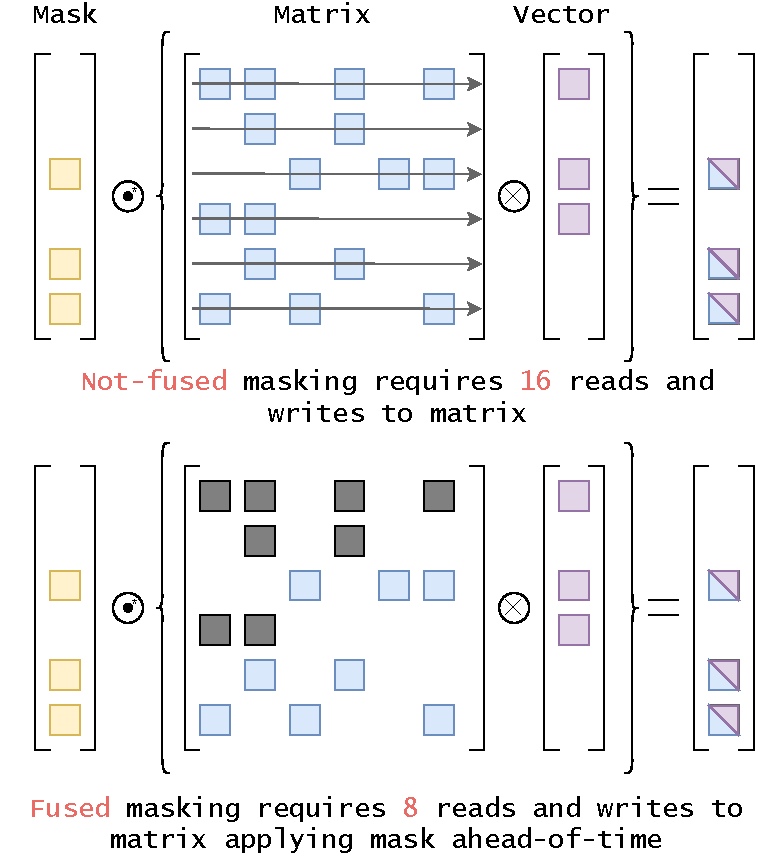
\includegraphics[width=0.99\textwidth]{MaskFusion.pdf}
\vspace{-1cm}
}


\headerbox {Motivation: Kernel fusion}
{name=matrices,column=0,span=8, row=1, below=CFPQ, bottomaligned=mask}%,bottomaligned=sol2}
{
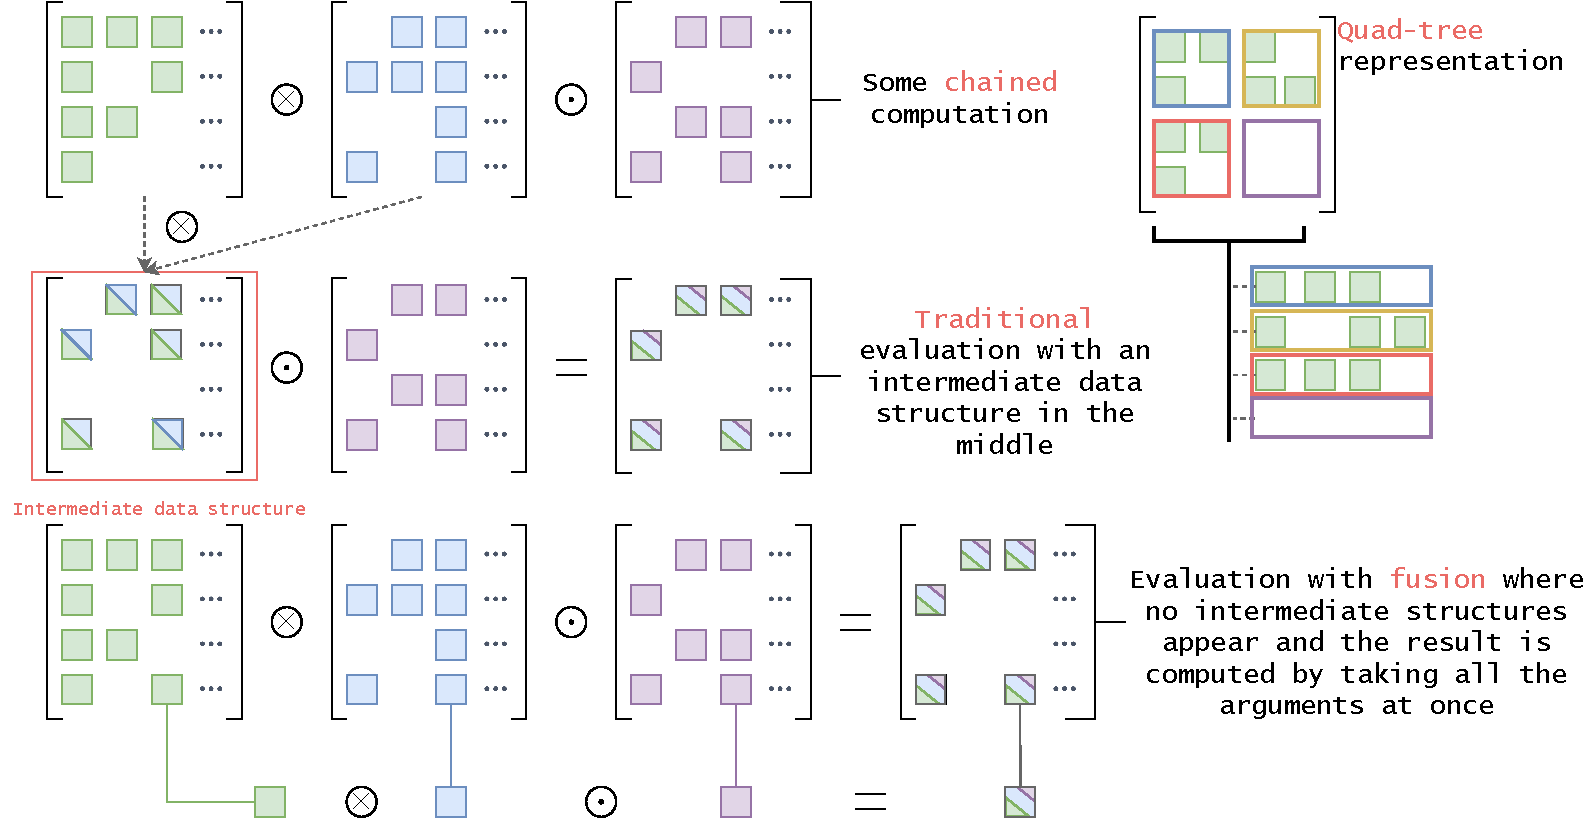
\includegraphics[width=\textwidth]{KernelFusion3.pdf}
}




% \setlength{\tabcolsep}{5pt}
% \headerbox{Evaluation: 2D Convolution}{name=scaling,span=7,column=3,row=2,below=rdfs}{
% \begin{minipage}[t]{0.26\textwidth}
%   \vspace{0pt}
% \textbf{Application}: data curving in cyber forensics. \\
% \textbf{Subject image}: random image  of size 1GB. \\
% \textbf{Filters}: random square filters with diameter 3 to 255.
% \end{minipage}
% \begin{minipage}[t]{0.37\textwidth}
%   \vspace{0pt}
%   \begin{overpic}[width=0.98\textwidth]{Conv_1070-crop}
%     \put (50,65) {{GTX-1070}}
%   \end{overpic}
% \end{minipage}
% \begin{minipage}[t]{0.37\textwidth}
%   \vspace{0pt}
%   \begin{overpic}[width=0.98\textwidth]{Conv_T4-crop}
%     \put (50,65) {{Tesla T4}}
%   \end{overpic}
% \end{minipage}
% \vspace{-0.1cm}
% }


\headerbox{Evaluation: Software}{name=rdfs, span=8, column=4, row=2, below=mask}{
%\vspace{0.05cm}
%\begin{table}[h]
%\rowcolors{1}{}{red}
% \begin{minipage}[t]{0.2\textwidth}
%   \vspace{0pt}
%   \hspace{2cm}
% % In $x / y$ $x$ stands for reductions and $y$ for memory accesses 
% \end{minipage}

% \begin{minipage}[t]{1\textwidth}
%   \vspace{0pt}
%     \centering
%     \begin{tabular}{ |c|c|c|c|c|c| } 
% \hline
% \multirow{2}{10em}{Function} & \multirow{2}{5em}{Description} & \multicolumn{3}{c}{\# of non-zeroes}\vline\\
% \cline{3-5}
% {}&{} & $10^1$ & $10^2$ & $10^3$ \\
% \hline
% \multirow{2}{10em}{E-wise successive additions} & Original & 1924 / 442 & 15876 / 2924 & 517312 / 83245\\ 
% & Distilled & 738 / 245 & 7755 / 2038 & 281103 / 66368\\
% \hline
% \multirow{2}{10em}{Kronecker with lower triangle masking} & Original & 5566 / 1143 & 44485 / 8121 & too large mask\\ 
% & Distilled & 2442 / 808 & 24213 / 6325 & too large mask\\
% \hline
% \multirow{2}{10em}{Kronecker with diagonal masking} & Original & 1377 / 246 & 1965 / 312 & 17595 / 2802\\ 
% & Distilled & 608 / 185 & 1166 / 239 & 10376 / 2129\\
% \hline
% \end{tabular}
% \end{minipage}
% \vspace{-0.1cm}
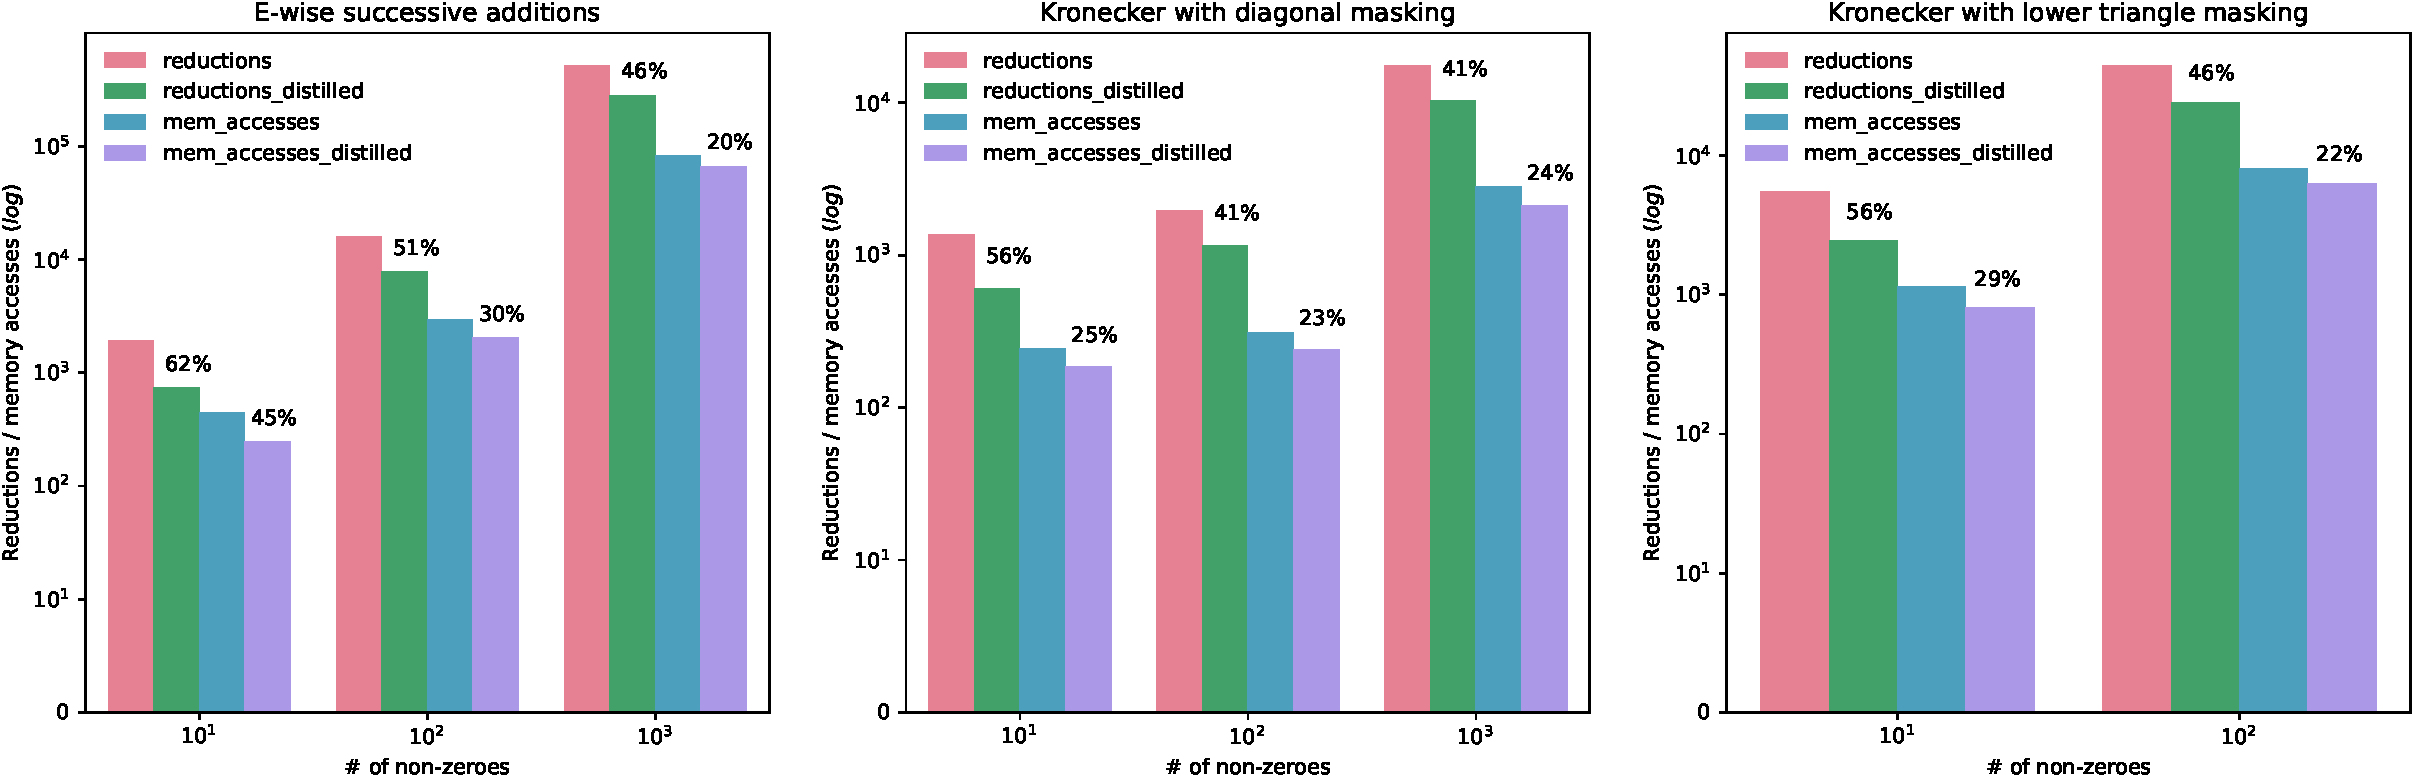
\includegraphics[width=\textwidth]{SoftwareBenchs3Cropped.pdf}
\vspace{-2.2cm}
}


\headerbox{Evaluation: Hardware}{name=hardware_eval, span=4, column=0, row=2, below=mask,bottomaligned=rdfs}{
%\vspace{0.05cm}
%\begin{table}[h]
%\rowcolors{1}{}{red}
% \begin{minipage}[t]{0.2\textwidth}
%   \vspace{0pt}
%   \hspace{2cm}
% % In $x / y$ $x$ stands for reductions and $y$ for memory accesses 
% \end{minipage}

% \begin{minipage}[t]{1\textwidth}
%   \vspace{0pt}
%     \centering
%     \begin{tabular}{ |c|c|c|c|c|c| } 
% \hline
% \multirow{2}{10em}{Function} & \multirow{2}{5em}{Description} & \multicolumn{3}{c}{\# of non-zeroes $^{3}$}\vline\\
% \cline{3-5}
% {}&{} & $30$ & $40$ & $70$ \\
% \hline
% \multirow{2}{10em}{E-wise successive additions} & Original & 1043 / 167 & 1345 / 207 & 1654 / 276\\ 
% & Distilled & 820 / 135 & 1044 / 175 & 1302 / 222\\
% \hline
% \end{tabular}
% \end{minipage}
% $^{3}$ such small smatrices are required due to some present technical limitation of FHW backend and to have the ability to count the numer of memory reads.
% \vspace{0.7cm}

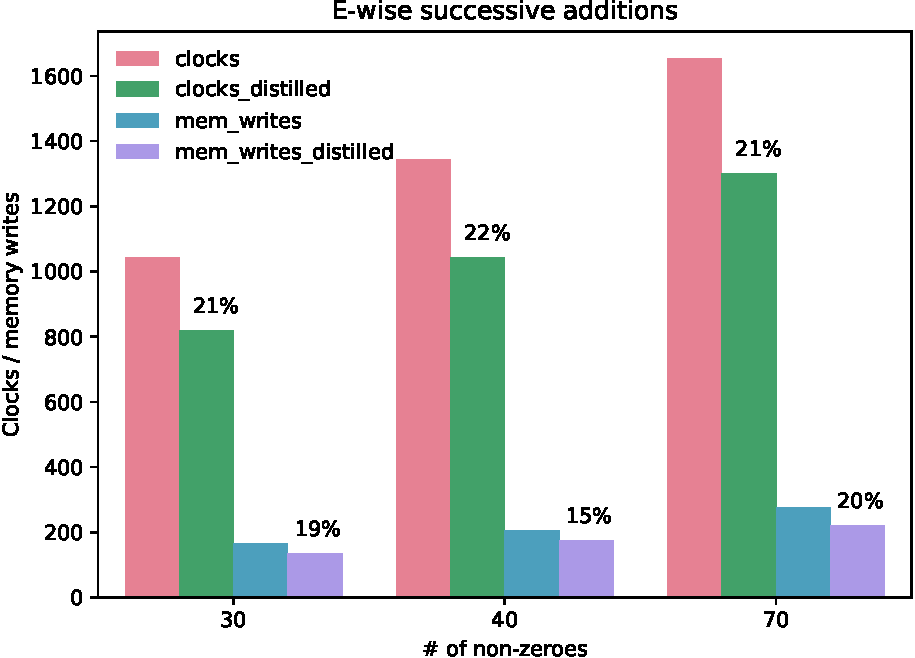
\includegraphics[width=0.9\textwidth]{HardwareBenchs2Cropped.pdf}
% \vspace{-1cm}

}


\headerbox{Implementation}{name=impl,span=4,column=0,row=3,below=hardware_eval}{
We use the distiller authored by Geoff Hamilton~\cite{distillation} and its functional language to evaluate the approach in terms of \textit{reductions} and \textit{memory accesses}.
\par

In order to provide both enough performance and interoperability with C++ (in which modern sparse frameworks are mostly written) we aim to synthesize a FPGA kernel from distilled functional program and utilize FHW project~\cite{Edwards2019FHWP} to do so.

}




% \headerbox {\smaller{Acknowledgments}}{name=ack,column=0,span=5,below=contact}{%bottomaligned=references
% \small
% This research was supported by Russian Foundation For Basic Research grant 18-01-00380, and a
% grant from JetBrains Research.
% }


\headerbox{\smaller{References}}{name=references,column=5,span=7,below=impl}{

    \scriptsize % Reduce the font size in this block
    \renewcommand{\section}[2]{\vskip 0.05em} % Get rid of the default "References" section title
    % \nocite{*} % Insert publications even if they are not cited in the poster
    \bibliographystyle{unsrt}
    \bibliographystyle{IEEEtran}
    \bibliography{main} % Use biblio.bib as the bibliography file
}


\headerbox {Results}{name=results,column=4,row=3, span=4,below=hardware_eval, bottomaligned=impl}{

  Distillation gives prominent results namely
  \begin{itemize}
    \item Shows up to \textbf{60\%} less reductions and \textbf{45\%} less memory accesses in software.
    \item Shows up to \textbf{20\%} less clock cycles and memory writes in hardware.
    % \item Also provides specialization and imposes a particular structure of the output programs which is more suitable for hardware generation.
  \end{itemize}  
}

\headerbox {Future Research}{name=answers,column=8,row=3, span=4,below=hardware_eval}{

  \begin{itemize}
    \item Moving the disiller from proof-of-concept to ready-to-use.
    \item Moving the hardware compiler from proof-of-concept to ready-to-use.
    \item Bridge the gap between our approach and existing sparse frameworks in a form of OpenCL-like kernels.
    \item Real-world examples evaluation.
  \end{itemize}

}


\headerbox {\smaller{Contact Us}}{name=contact,column=0,span=5,below=impl,bottomaligned=references}{
\small
\begin{minipage}[t]{0.75\textwidth}
  \vspace{0pt}
Our team:
\begin{itemize}
  \item Aleksey Tyurin: \href{mailto:alekseytyurinspb@gmail.com}{alekseytyurinspb@gmail.com}
  \item Daniil Berezun: \href{mailto:daniil.berezun@jetbrains.com}{daniil.berezun@jetbrains.com}
  \item Ekaterina Vinnik: \href{mailto:catherine.vinnik@gmail.com}{catherine.vinnik@gmail.com}
  \item Semyon Grigorev: \href{mailto:s.v.grigoriev@spbu.ru}{s.v.grigoriev@spbu.ru}
\end{itemize}

\end{minipage}
~
\begin{minipage}[t]{2cm}
  \vspace{0pt}

\includegraphics[width=2cm]{jbr-gpuSpec.pdf}
\end{minipage}

}

\end{poster}


\end{document}
